% !TEX TS-program = xelatex
% !TEX encoding = UTF-8 Unicode
\documentclass[10pt,aspectratio=1610]{beamer}
%\documentclass[10pt]{beamer}

\usetheme[progressbar=frametitle]{metropolis}
\usepackage{appendixnumberbeamer}


\usepackage{booktabs}
\usepackage[scale=2]{ccicons}

\usepackage{pgfplots}
\usepgfplotslibrary{dateplot}

\usepackage{xspace}

\usepackage{bm}

% Color definitions 
%\usepackage[dvipsnames]{xcolor}

% Remove "Figure #" from figures
\setbeamertemplate{caption}{\raggedright\insertcaption\par}

% Custom commands
% Metropolis theme name 
\newcommand{\themename}{\textbf{\textsc{metropolis}}\xspace}

% Derivatives
\newcommand{\pfrac}[3][]{\frac{\partial^{#1} #2}{\partial #3^{#1}}}
\newcommand{\dd}[3][]{\frac{\mathrm{d}^{#1} #2}{\mathrm{d} #3^{#1}}}
\newcommand{\pp}[2][]{\partial^{#1}_{#2}}


\newcounter{example}
\stepcounter{example}
\newcounter{exercise}
\stepcounter{exercise}

\renewcommand{\vec}{\mathbf}
\newcommand{\varone}{\vec{x}}
\newcommand{\argone}{(t,\varone)}
\newcommand{\R}{\mathbb{R}}
\newcommand{\CC}{\mathbb{C}}
\newcommand{\Q}{\mathbb{Q}}
\newcommand{\Z}{\mathbb{Z}}
\newcommand{\N}{\mathbb{N}}
\newcommand{\norm}[1]{\left\lVert#1\right\rVert}
\newcommand{\fone}{\vec{f}}
\newcommand{\ftwo}{\vec{g}}
\newcommand{\fthr}{\vec{h}}
\newcommand{\ffor}{\bm{\phi}}
\newcommand{\opone}{\mathcal{L}}
\newcommand{\optwo}{\mathcal{G}}
\renewcommand{\Re}{\operatorname{Re}}
\newcommand{\iprod}[2]{\langle #1,#2 \rangle}
\newcommand{\diff}{\mathrm{d}}
\newcommand{\fouriert}{\mathcal{F}}

\title{Boundary conditions}
\subtitle{Some basic properties and more specific questions}
\date{16/2/2021}
\date{}
%\author{18.303 Linear Partial Differential Equations: Analysis and Numerics}
\institute{18.303 Linear Partial Differential Equations: Analysis and Numerics}
\titlegraphic{\hfill
\includegraphics[height=2em]{../MIT-logo.pdf}}

\begin{document}
	
	\maketitle
	
%	\begin{frame}{Table of contents}
%		\setbeamertemplate{section in toc}[sections numbered]
%		\tableofcontents%[hideallsubsections]
%	\end{frame}

%%%%%%%%%%%%%%%
%\section{Finite differences}
%%%%%%%%%%%%%%%

\begin{frame}{Basic Notions}
	\begin{columns}[T,onlytextwidth]
		\column{0.46\textwidth}
		Boundary value problems look basically like this:
		\[ 
		\begin{split}
			\opone u(\varone) &= f(\varone), \; \varone \in \Omega; \\ 
			\optwo u(\varone) &= g(\varone), \; \varone \in \partial \Omega.
		\end{split}
		 \]
		 
		\onslide*<1>{Now, if $ \fone = 0$, we say that the boundary value problem (the differential equation) is \alert{homogeneous}. Otherwise the problem is said to be \alert{inhomogeneous}.}
		
		\onslide<2->{If the differential operator $ \optwo $ is just a (non-zero) function, these are \alert{Dirichlet boundaries} and $ u $ is equal to some function on the boundary $ \partial \Omega $.}
		
		\onslide<3->{If the differential operator is $ \nvec \cdot \nabla = \pfrac{}{\nvec} $ the boundary condition is called \alert{Neumann type} or \alert{flux boundary} condition. This denotes the derivative of function $ u $ in the normal direction of the boundary given by the normal vector $ \nvec (\varone) $ (note that generally it depends on the point $ x \in \partial \Omega$).}
		
		\column{0.08\linewidth}
		\column{0.46\textwidth}
		\vspace{4em}
		\begin{figure}
			\centering
			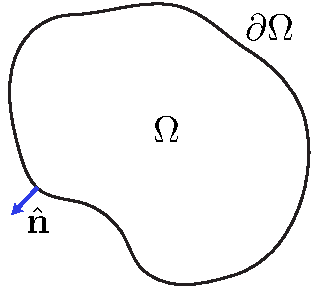
\includegraphics[width=0.8\linewidth]{domain.pdf}
			\caption{An example of a 2d domain and its boundary.}
		\end{figure}
	\end{columns}
\end{frame}

\begin{frame}
	Boundary conditions can be more complicated than Dirichlet or Neumann conditions (and will be e.g. for higher order differential operators). However, we have the following general property:
	
	Let $ u_0(\varone) $ solve the \emph{homogeneous} problem
	\[ \begin{split}
		\opone u_0(\varone) &= 0, \; \varone \in \Omega; \\ 
		\optwo u_0(\varone) &= g(\varone), \; \varone \in \partial \Omega.
	\end{split} \]
	
	Now, consider the function $ u(\varone) = v(\varone) + u_0(\varone). $ We have 
	\[ \opone u(\varone) = \opone v(\varone) + \underbrace{\opone u_0 (\varone)}_{=0} = f(\varone). \]
	
	We notice that it suffices to require that 
	\[ \optwo v(\varone) = 0,\; \varone \in \partial \Omega \]
	 because this will make sure that $ \optwo u(\varone) = g(\varone) $, when $ \varone \in \partial \Omega $.
\end{frame}

\begin{frame}
	Now we have a boundary value problem 
	\[ \begin{split}
		\opone v(\varone) &= f(\varone), \; \varone \in \Omega; \\ 
		\optwo v(\varone) &= 0, \; \varone \in \partial \Omega.
	\end{split} \]

	This shows us that the general solution can be sought as \\ \alert{the solution to the homogeneous problem with inhomogeneous boundaries} + \alert{the solution to the inhomogeneous problem with homogeneous boundaries}.
\end{frame}

\begin{frame}{Exercise \exercisen}
	How would you modify the solution to the zero boundary condition Poisson equation to solve
	\[ \begin{split}
		\pfrac[2]{u(\varone)}{x} &= f(x),\; x\in [0,1]; \\
		u(0)&=1,\; u(1) = 2?
	\end{split} \]
\end{frame}

\begin{frame}{Finite differences revisited}
	Remember that we talked about the difficulty of defining matrix operations corresponding to the \alert{finite difference} approximations of continuous differential operators. 
	
	As ar reminder, consider the Laplacian operator with a finite difference approximation
	 \[ \delta^{(2)} \vec{u} = \frac{1}{\Delta x^2}\begin{pmatrix}
		u_0 - 2 u_1 + u_2 \\ u_1 - 2 u_2 + u_3 \\  \vdots \\ u_{N-1} - 2u_{N} + u_{N+1}
	\end{pmatrix}. \] 

	Here $ u_k = u(k \Delta x) $, where $ i=1,2,3,...,N $ ($ u \in [0,1]) $ and the discretization is given by $ \Delta x = 1/(N+1) $. 
\end{frame}

\begin{frame}
	An alternative way of looking at this with different boundaries is by defining the functions that we are interested in the open interval, say $ x \in (0,1) = \Omega$. We have the boundary $ \partial \Omega = \{0,1\} $ consisting of just two points. 
	
	The overall domain for $ u $ is given by the closure $ \overline{\Omega} $. We can extend the discretized version to include the boundary points $ u_0 $ and $ u_{N+1} $. 
	
	Assume we have zero Dirichlet boundaries. Now we just set our extended operator to 
	\[ \delta^{(2)}_{\text{D}} = \frac{1}{\Delta x^2} \begin{pmatrix}
		0 & \dots & & & & & \\
		1 & -2 & 1  &   & &  &  \\
		 & 1  & -2 & 1 &  &  & \\
		& & \ddots & \ddots & \ddots  & & \\
		& & & 1 & -2 & 1 & \\
		& & & & 1 & -2 & 1 \\
		& & & & & \dots & 0
	\end{pmatrix} \in \R^{N+2 \times N+2}. \]
\end{frame}

\begin{frame}
	\alert{Word of warning:} This operator cannot be inverted. It is only possible to solve for the interior points. If this system is solved, we still need the extra information that $ u_0 = u_{N+1} = 0 $. 
	
	\pause
	\textbf{Question:} how would you modify the matrix to account for $ u'(0) = u'(1) = 0 $ (Neumann condition)?
	
	\pause
	\textbf{Answer:} If $ u_0 = u_1 $ and $ u_{N+1} = u_N $, suitable finite differences (forward and backward, respectfully) give $ u'(0) = u'(1) = 0 $ i.e. 
	\[ \delta^{(2)}_{\text{N}} = \frac{1}{\Delta x^2} \begin{pmatrix}
		1 & -2 & 1 & 0  & \dots & & & \\
		1 & -2 & 1  &   & &  &  \\
		& 1  & -2 & 1 &  &  & \\
		& & \ddots & \ddots & \ddots  & & \\
		& & & 1 & -2 & 1 & \\
		& & & & 1 & -2 & 1 \\
		& & \dots & 0 & 1 & -2 & 1
	\end{pmatrix} \in \R^{N+2 \times N+2}. \]
\end{frame}

\begin{frame}
	Often this is implemented on a computer by not caring about the first and last rows of the matrix but setting boundaries explicitly after calculating the Laplacian $ \Delta u(x) $.
	
	In practice this gives us an operation 
	\[ \delta^{(2)} = \frac{1}{\Delta x^2} \begin{pmatrix}
		1 & -2 & 1  &   & &  &  \\
		& 1  & -2 & 1 &  &  & \\
		& & \ddots & \ddots & \ddots  & & \\
		& & & 1 & -2 & 1 & \\
		& & & & 1 & -2 & 1 
	\end{pmatrix} \in \R^{N \times N+2} \]
	That calculates the interior points from $ k=1,..,N $ given an input $ \vec{u} \in \R^{N+2} $ with the proper boundary points. 
	
	Remember that we can't define higher order difference operations using just nearest neighbors (recall e.g. the polynomial fitting method). This shows that for higher order operators we need more boundary points. 
\end{frame}

\begin{frame}
	\textbf{Question:} how would you define the matrix for periodic boundaries? 
	
	\pause
	\textbf{Answer:} For periodic boundaries we have 
	\[ \delta^{(2)}_{\text{p}} = \frac{1}{\Delta x^2} \begin{pmatrix}
		-2 & 1 & 0 & \dots  &  & & 1 \\
		1 & -2 & 1  &   & &  &  \\
		& 1  & -2 & 1 &  &  & \\
		& & \ddots & \ddots & \ddots  & & \\
		& & & 1 & -2 & 1 & \\
		& & & & 1 & -2 & 1 \\
		-2 & 1 &  &  & \dots & 0 & 1
	\end{pmatrix} \in \R^{N+2 \times N+2}. \]
\end{frame}

\begin{frame}
	However, periodic boundary conditions are a special case because in practice there are no two boundaries but just one special boundary. This can be seen from the previous matrix that has only one redundant row (the last one). 
	
	\pause
	This is why we normally work with the periodic Laplacian 
	\[ \delta^{(2)}_{\text{p}} = \frac{1}{\Delta x^2} \begin{pmatrix}
		-2 & 1 & 0 & \dots  &  & & 1 \\
		1 & -2 & 1  &   & &  &  \\
		& 1  & -2 & 1 &  &  & \\
		& & \ddots & \ddots & \ddots  & & \\
		& & & & 1 & -2 & 1  \\
		1 & & & & & 1 & -2 
	\end{pmatrix} \in \R^{N+1 \times N+1} \]
	that operates on values $ u(k \Delta x) $, where $ k=0,1,2,...,N $.  Now the boundary gives the extension to one point $ u(1) = u((N+1)\Delta x) = u(0) $. 
	
	\pause
	\textbf{Question:} Is this operator invertible?
\end{frame}

\end{document}
